% use the standard article class with 12pt font
\documentclass[12pt]{article}

% load a minimal set of packages packages
\usepackage{fullpage}
\usepackage{setspace}
\usepackage{graphicx}
\usepackage{natbib}
\usepackage{amsmath}
\usepackage{amsfonts}
\usepackage{amssymb}
\usepackage{hyperref}
\bibpunct{(}{)}{;}{a}{}{,}

% set custom paragraph spacing 
\parskip=0pt
\parindent=20pt

% create footnote command so that my name
% has an asterisk rather than a one.
\long\def\symbolfootnote[#1]#2{\begingroup%
\def\thefootnote{\fnsymbol{footnote}}\footnote[#1]{#2}\endgroup}

% set up references. eliminate distracting boxes and colors.
\hypersetup{
  colorlinks=true, % false: boxed links; true: colored links
  linkcolor=black, % color of internal links
  citecolor=black, % color of links to bibliography
  filecolor=blue, % color of file links
  urlcolor=blue % color of external links
}

% begin the document
\begin{document}

% insert title manually (personal preference)
\begin{center}
{\LARGE \textbf{Titley}}\\\vspace{2mm}
{ \textbf{Subtitle}}\symbolfootnote[1]{Thanks to everyone who helped me.}

\vspace{5mm}

Carlisle Rainey\symbolfootnote[2]{Carlisle Rainey is ...}
\end{center}

\vspace{5mm}

% abstract
{\centerline{\textbf{Abstract}}}
\begin{quote}
\noindent Put the abstract here...
\end{quote}

% remove page number from first page
\thispagestyle{empty}

% start main text
\doublespace

Start the introduction here...

\section*{A Heading}

Continue here...

\subsection*{A Sub-Heading}

Continue...

\section*{A Figure}

% add the figure
\begin{figure}[h!]
\begin{center}
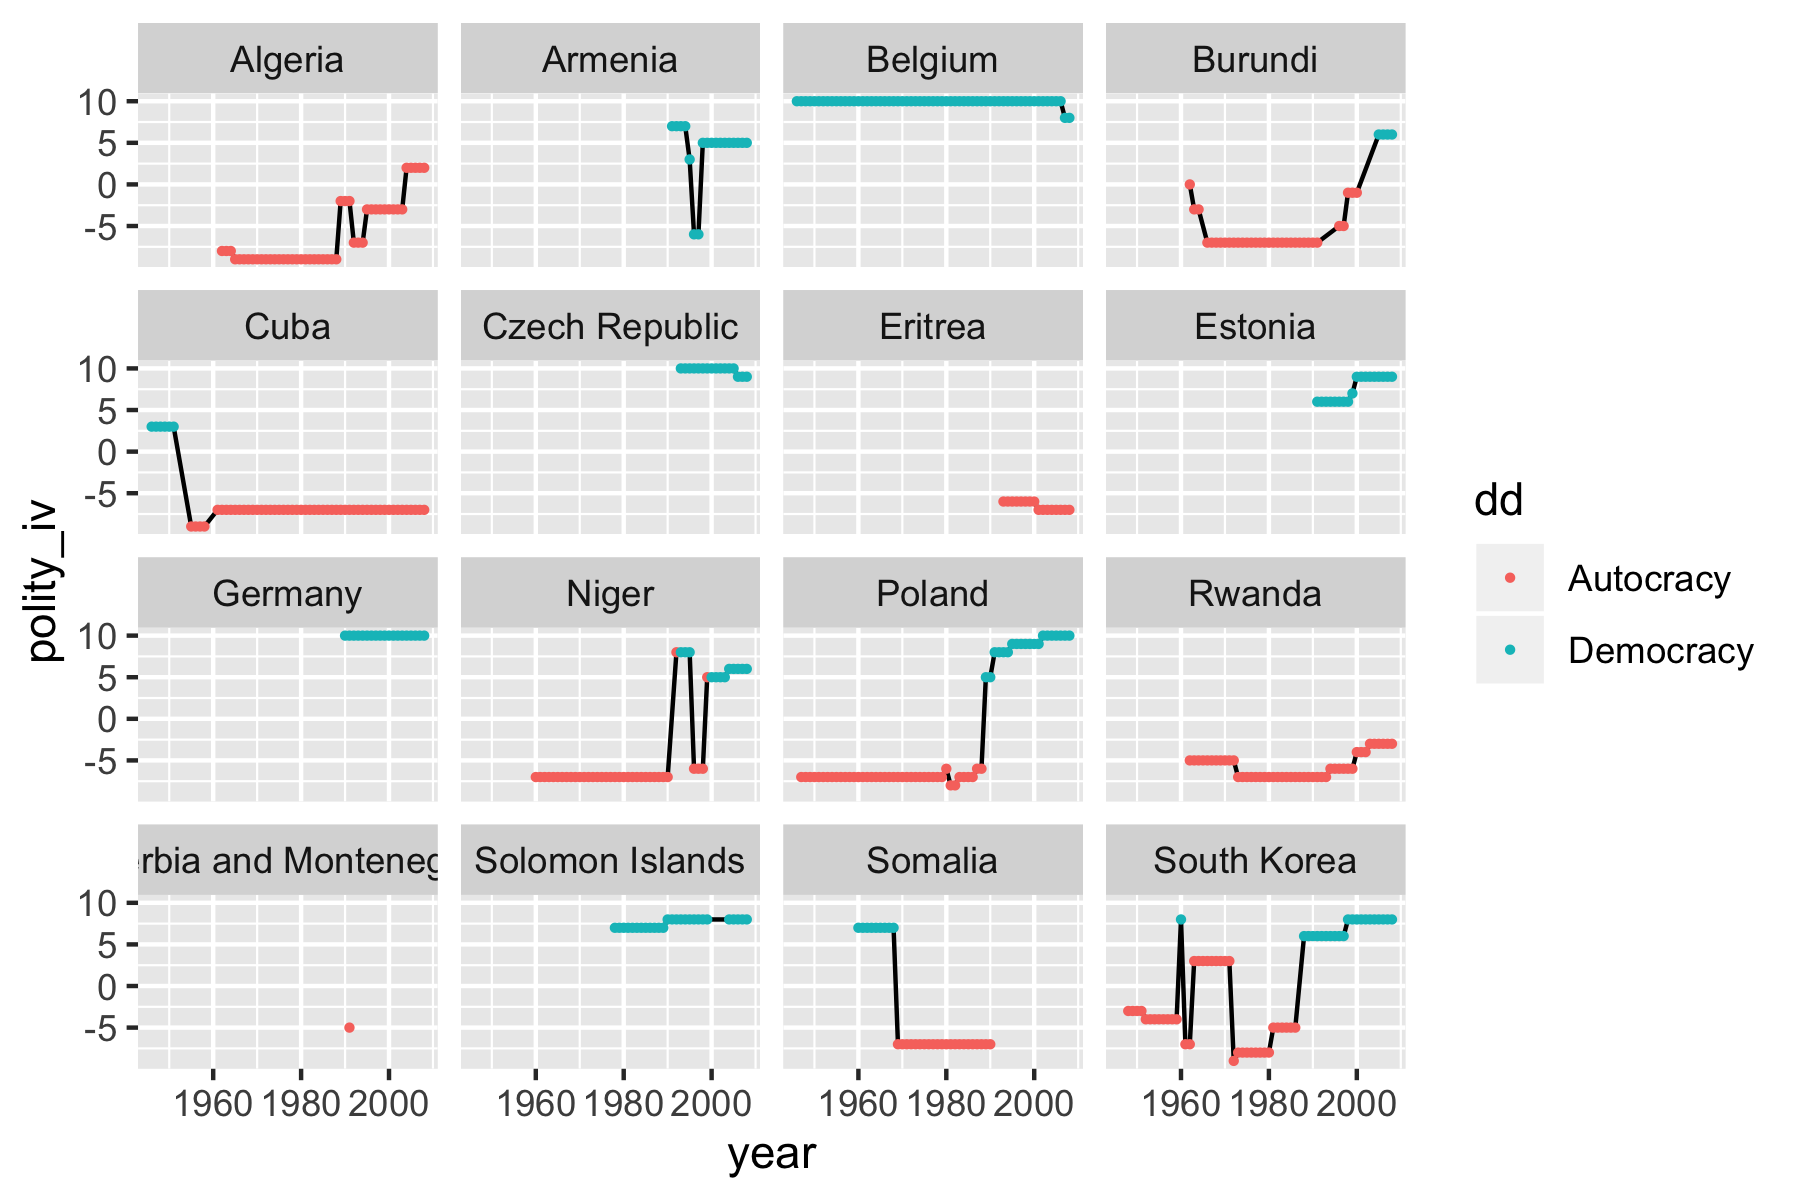
\includegraphics[width = \textwidth]{fig/plot1.png}
\caption{This figure shows something really interesting.}\label{fig:something-interesting}
\end{center}
\end{figure}


\section*{An (Ugly) Table}


\begin{tabular}{l|r|r|r|r|r|r}
\hline
term & estimate & std.error & statistic & p.value & conf.low & conf.high\\
\hline
(Intercept) & -1.4428278 & 0.0649491 & -22.21476 & 0 & -1.572885 & -1.3181194\\
\hline
polity\_iv & 0.4576718 & 0.0102670 & 44.57678 & 0 & 0.438014 & 0.4782861\\
\hline
\end{tabular}


\end{document}


